\documentclass[twocolumn]{aastex61}
%\usepackage{geometry}                		% See geometry.pdf to learn the layout options. There are lots.
%\geometry{letterpaper}                   		% ... or a4paper or a5paper or ... 
%\geometry{landscape}                		% Activate for for rotated page geometry
\usepackage{graphicx}				% Use pdf, png, jpg, or eps with pdflatex; use eps in DVI mode
								% TeX will automatically convert eps --> pdf in pdflatex		
\usepackage{amssymb}
\usepackage{color}
\usepackage{amsmath}
\usepackage[bottom]{footmisc}

\usepackage{natbib}
\bibliographystyle{apj}

\newcommand{\zfourge}{{\sc zfourge}}
\newcommand{\Hbeta}{H$\beta$}
\newcommand{\OIII}{[\hbox{{\rm O}\kern 0.1em{\sc iii}}]}
\newcommand{\Ks}{$K_s$}
\newcommand{\Av}{A$_{\rm V}$}

\shortauthors{Forrest et al.}

\begin{document}

\title{The Long and Illustrious Title of the Article, Which Somehow is Simultaneously Concise and Unassuming at $\MakeLowercase{z} \sim 0$\footnote{This paper includes data gathered with the 6.5 meter Magellan Telescopes located at Las Campanas Observatory, Chile.}}

\correspondingauthor{}
\email{username@physics.tamu.edu}

%\author[ORCiD]{Name}
\author{My Name}
\affiliation{George P. and Cynthia W. Mitchell Institute for Fundamental Physics and Astronomy, Department of Physics and Astronomy, Texas A\&M University, College Station, TX 77843, USA}



\begin{abstract}

\zfourge ZFOURGE
Here we have our succinct abstract with no references in a single paragraph.
Blah blah blah blah blah blah blah blah blah blah blah blah blah blah blah blah blah blah blah blah blah blah blah blah blah blah blah blah blah blah blah blah blah blah blah blah blah blah blah blah blah blah blah blah blah blah blah blah blah blah blah blah blah blah blah blah blah blah blah blah blah blah blah blah blah blah blah blah blah blah blah blah blah blah blah blah blah blah blah blah blah blah blah blah blah blah blah blah blah blah blah blah blah blah blah blah blah blah blah.

\end{abstract}


\keywords{galaxies: evolution --- galaxies: formation --- galaxies: high-redshift --- galaxies: starburst --- large-scale structure of universe --- ultraviolet: galaxies}


\section{Introduction}


Background information and literature review with SOOOOO many references. 
Show off how much you've read.
I can cite a paper as found in \citet{Straatman2016}, or I can add the reference parenthetically \citep[e.g.,][hereafter F16]{Alcorn2016, Forrest2016}.
I like put each sentence on its own line.
You need two returns to start a new paragraph.

Some people prefer to have all of the lines in their 
LaTeX file the same length, ignoring where new
sentences start.  Whatever works for you is fine, as
long as you can easily find where errors are or
where pieces that need fixing exist.

New commands, like \OIII\ are really useful and can save a lot of typing relative to [\hbox{{\rm O}\kern 0.1em{\sc iii}}].
Compare \OIII\ to \OIII and \OIII.

Blah blah blah blah blah blah blah blah blah blah blah blah blah blah blah blah blah blah blah blah blah blah blah blah blah blah blah blah blah blah blah blah blah blah blah blah blah blah blah blah blah blah blah blah blah blah blah blah blah blah blah blah blah blah blah blah blah blah blah blah blah blah blah blah blah blah blah blah blah blah blah blah blah blah blah blah blah blah blah blah blah blah blah blah blah blah blah blah blah blah blah blah blah blah blah blah blah blah blah.


\section{Data \& Methods} \label{Methods}

Blah blah blah blah blah blah blah blah blah blah blah blah blah blah blah blah blah blah blah blah blah blah blah blah blah blah blah blah blah blah blah blah blah blah blah blah blah blah blah blah blah blah blah blah blah blah blah blah blah blah blah blah blah blah blah blah blah blah blah blah blah blah blah blah blah blah blah blah blah blah blah blah blah blah blah blah blah blah blah blah blah blah blah blah blah blah blah blah blah blah blah blah blah blah blah blah blah blah blah.


\subsection{Subsection}

Blah blah blah blah blah blah blah blah blah blah blah blah blah blah blah blah blah blah blah blah blah blah blah blah blah blah blah blah blah blah blah blah blah blah blah blah blah blah blah blah blah blah blah blah blah blah blah blah blah blah blah blah blah blah blah blah blah blah blah blah blah blah blah blah blah blah blah blah blah blah blah blah blah blah blah blah blah blah blah blah blah blah blah blah blah blah blah blah blah blah blah blah blah blah blah blah blah blah blah.


\subsection{Subsection}

Blah blah blah blah blah blah blah blah blah blah blah blah blah blah blah blah blah blah blah blah blah blah blah blah blah blah blah blah blah blah blah blah blah blah blah blah blah blah blah blah blah blah blah blah blah blah blah blah blah blah blah blah blah blah blah blah blah blah blah blah blah blah blah blah blah blah blah blah blah blah blah blah blah blah blah blah blah blah blah blah blah blah blah blah blah blah blah blah blah blah blah blah blah blah blah blah blah blah blah.


%-----------------------------------------------------   
\begin{table}[t]
  \centering
  \caption{This is the table caption.}}
  \label{tab:table1}
  \begin{tabular}{l | c | c}	%alignment in columns (left-l [ell], center-c, right-r, vertical line-| [vertical line])
	   & Column A & Column B\\
	 \hline \hline
	Object A	& 1 		& 3 \\
	Object B	& 3 		& 6 \\
	Object C	& 7 		& 1 \\
	Object D   & 2		& 2 \\
	\hline
	Total\footnote{Footnote A.}  & 13 & 12 \\
  \end{tabular}
\end{table}
%-----------------------------------------------------   


\section{Some Analysis or Something}

We can reference Section \ref{Methods} and Table \ref{tab:table1} if we want.
Blah blah blah blah blah blah blah blah blah blah blah blah blah blah blah blah blah blah blah blah blah blah blah blah blah blah blah blah blah blah blah blah blah blah blah blah blah blah blah blah blah blah blah blah blah blah blah blah blah blah blah blah blah blah blah blah blah blah blah blah blah blah blah blah blah blah blah blah blah blah blah blah blah blah blah blah blah blah blah blah blah blah blah blah blah blah blah blah blah blah blah blah blah blah blah blah blah blah blah.

%-----------------------------------------------------

	\begin{figure}[t]
	\centerline{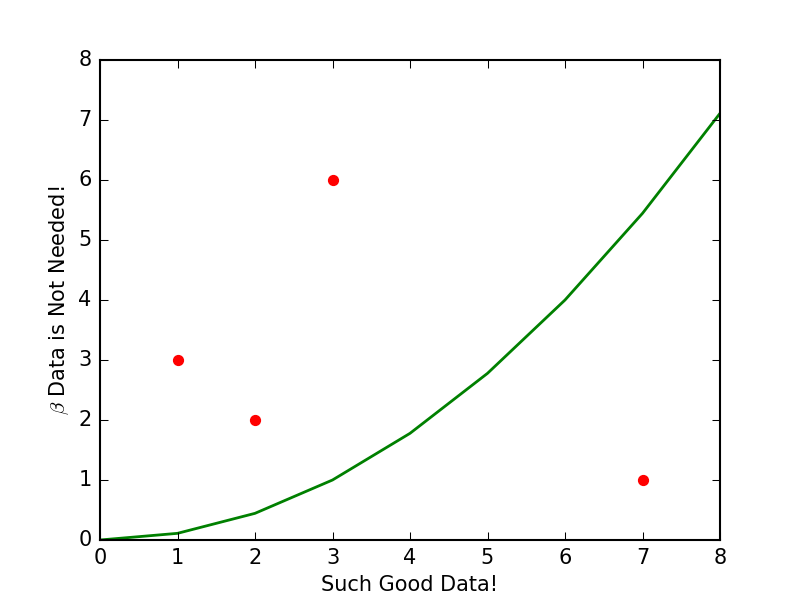
\includegraphics[width=0.5\textwidth, trim=0in 0in 0in 0in, clip=true]{figure_1.png}}
	\caption{This is my figure caption.}
	\label{fig:figure1}
	\end{figure}

%-----------------------------------------------------  



%-----------------------------------------------------

	\begin{figure*}[t]
	\centerline{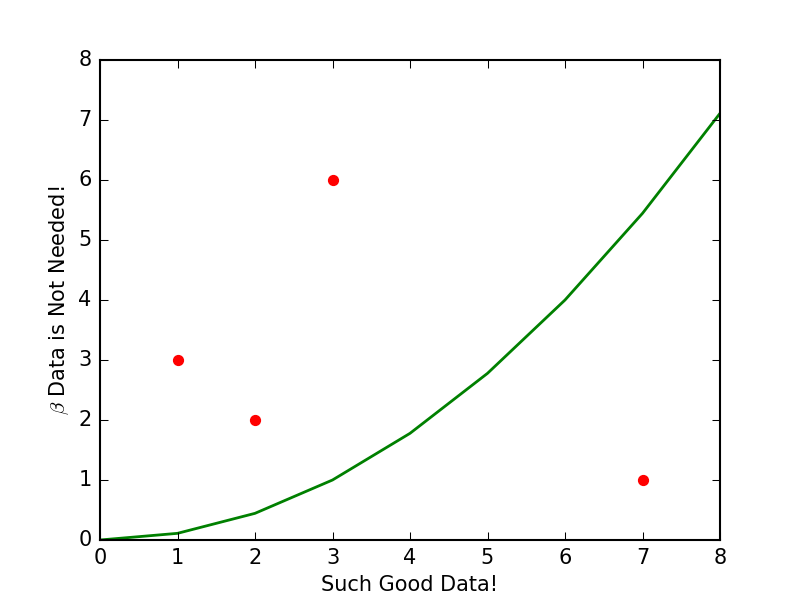
\includegraphics[width=\textwidth, trim=0in 0in 0in 0in, clip=true]{figure_1.png}}
	\caption{Or span both columns...}
	\label{fig:figure2}
	\end{figure*}

%-----------------------------------------------------  

\subsection{Mere detailed section?}

Blah blah blah blah blah blah blah blah blah blah blah blah blah blah blah blah blah blah blah blah blah blah blah blah blah blah blah blah blah blah blah blah blah blah blah blah blah blah blah blah blah blah blah blah blah blah blah blah blah blah blah blah blah blah blah blah blah blah blah blah blah blah blah blah blah blah blah blah blah blah blah blah blah blah blah blah blah blah blah blah blah blah blah blah blah blah blah blah blah blah blah blah blah blah blah blah blah blah blah.


\subsection{Section titles are deteriorating quickly}

Blah blah blah blah blah blah blah blah blah blah blah blah blah blah blah blah blah blah blah blah blah blah blah blah blah blah blah blah blah blah blah blah blah blah blah blah blah blah blah blah blah blah blah blah blah blah blah blah blah blah blah blah blah blah blah blah blah blah blah blah blah blah blah blah blah blah blah blah blah blah blah blah blah blah blah blah blah blah blah blah blah blah blah blah blah blah blah blah blah blah blah blah blah blah blah blah blah blah blah.

We use $F=\lambda^\beta$ for our work, or pull it out of line with $$F=\lambda^\beta$$.

Alternatively, we can put a number of equations together,
\begin{eqnarray}
F=\lambda^\beta\\
2=4
\end{eqnarray}

align them, 
\begin{eqnarray}
F&=&\lambda^\beta\\
2&=&4
\end{eqnarray}

and remove numbers if we so choose.
\begin{eqnarray*}
F&=&\lambda^\beta\\
2&=&4
\end{eqnarray*}


\subsection{Something something something DARK SIDE}

It is a period of civil war.
Rebel spaceships, striking
from a hidden base, have won
their first victory against
the evil Galactic Empire.

During the battle, Rebel
spies managed to steal secret
plans to the Empire's
ultimate weapon, the DEATH
STAR, an armored space
station with enough power
to destroy an entire planet.

Pursued by the Empire's
sinister agents, Princess
Leia races home aboard her
starship, custodian of the
stolen plans that can save her
people and restore
freedom to the galaxy....



\section{Conclusions}

Blah blah blah blah blah blah blah blah blah blah blah blah blah blah blah blah blah blah blah blah blah blah blah blah blah blah blah blah blah blah blah blah blah blah blah blah blah blah blah blah blah blah blah blah blah blah blah blah blah blah blah blah blah blah blah blah blah blah blah blah blah blah blah blah blah blah blah blah blah blah blah blah blah blah blah blah blah blah blah blah blah blah blah blah blah blah blah blah blah blah blah blah blah blah blah blah blah blah blah.

We found something!
   
   
\section*{Acknowledgments}


We wish to thank the Mitchell family, particularly the late George P. Mitchell, for their continuing support of astronomy.
The referee was super chill.
Peace, bro!







\bibliography{library}


\end{document}



